---
id: tkz-euclide-ejemplo-19
title: "Ángulos"
description: "Rellena, marca y etiqueta la amplitud de un ángulo dado."
keywords: [angulos, medida, marcado, relleno]
tags: [tkzFillAngle,tkzMarkAngle,tkzLabelAngle]
sort: 19
---
\documentclass[tikz,border=2mm]{standalone}
\usepackage{tkz-base}
\usepackage{tkz-euclide}

\begin{document}
    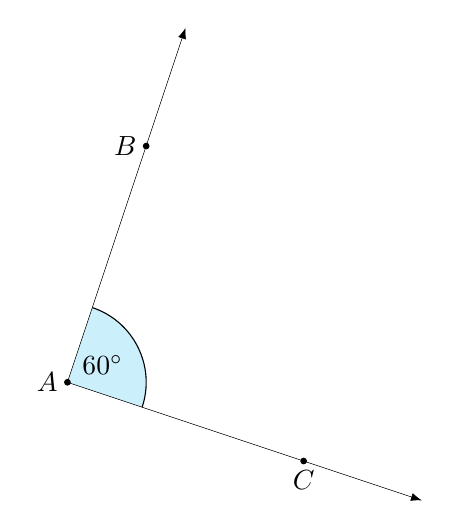
\begin{tikzpicture}
        % Define puntos A,B,C,D
        \tkzDefPoints{
            2/1/A,
            3/4/B,
            5/0/C%
        }

        % Rellena ángulo ∠CAB de color cyan
        \tkzFillAngle[size=1,cyan!20](C,A,B)
        % Marca el ángulo ∠CAB
        \tkzMarkAngle[size=1](C,A,B)
        % Etiqueta el ángulo ∠CAB como 60°
        \tkzLabelAngle[pos=0.5](C,A,B){$60^{\circ}$}

        % Dibuja los puntos A,B,C
        \tkzDrawPoints(A,B,C)

        % Dibuja las rectas AB y AC
        \tkzDrawLines[-Latex,add=0 and .5](A,B A,C)

        % Etiqueta los puntos en posiciones convenientes.
        \tkzLabelPoints[left](A,B)
        \tkzLabelPoints[below](C)
    \end{tikzpicture}
\end{document}
